% ds-instruc-07.tex

%-------------------------------------------------------------------------
\documentclass[11pt,a4paper]{article}
%-------------------------------------------------------------------------

%-------------------------------------------------------------------------
%-------------------------------------------------------------------------
% ds-info-S1-preambule.tex
%-------------------------------------------------------------------------

%-------------------------------------------------------------------------
\usepackage{calc}
\usepackage[text={16cm,23cm},centering=true,showframe=false]{geometry}
\usepackage{fancybox,fancyvrb,fancyhdr,lastpage,lineno,import}
\usepackage{longtable,multirow}
\usepackage{xcolor,graphics,xmpmulti,pgf,pgfpages,tikz,wrapfig}
\usepackage{colortbl,color}
\usepackage{amsmath,amssymb,amsfonts}
\usepackage{hyperref,multimedia,rotating,framed,pstricks}
\usepackage{listings,index}
%
%---- pdflatex
%\usepackage[T1]{fontenc}
%\usepackage[utf8]{inputenc}
%---- xelatex
\usepackage{fontspec}
%
%\usepackage[french]{minitoc}
\usepackage[french]{babel}
\usepackage[french]{nomencl}
\usepackage[framed,hyperref,standard]{ntheorem}
\usepackage{eurosym,pifont}
%-------------------------------------------------------------------------

%-------------------------------------------------------------------------
\lstset
{
language=Python,
basicstyle=\ttfamily,
identifierstyle=\ttfamily,
keywordstyle=\color{blue}\ttfamily,
commentstyle=\color{gray}\ttfamily,
stringstyle=\color{green}\ttfamily,
showstringspaces=false,
extendedchars=true,
numbers=left, 
numberstyle=\color{blue}\tiny,
frame=lines,
linewidth=0.95\textwidth,
xleftmargin=5mm
} 
%-------------------------------------------------------------------------

%-------------------------------------------------------------------------
\pgfdeclareimage[width=3cm,interpolate=true]{logo-enib}{logo-enib}
%-------------------------------------------------------------------------

%-------------------------------------------------------------------------
\pagestyle{fancy}
\fancyhead{}
\fancyhead[L]{\hspace*{-3em}\begin{minipage}{3cm}\pgfuseimage{logo-enib}\end{minipage}}
\fancyhead[C]{Informatique S1}
\fancyhead[R]{\thepage/\pageref{LastPage}}
\fancyfoot{}
\fancyfoot[L]{}
\fancyfoot[C]{}
\fancyfoot[R]{}
\setlength{\headheight}{80pt}
\setlength{\footskip}{38pt}
\renewcommand{\headrulewidth}{0pt}
\renewcommand{\footrulewidth}{0pt}
%-------------------------------------------------------------------------

\voffset=-1cm

%-------------------------------------------------------------------------
\def\entete{\noindent\begin{tabular}{|l|l|l|} 
\hline 
 & & \\ 
\makebox[6cm][l]{\bsc{Nom :}} & \makebox[6cm][l]{\bsc{Prénom :}} & \makebox[2.65cm][l]{\bsc{Groupe :}} \\[1mm] 
\hline 
\end{tabular}\\[1mm]
{\footnotesize \textsc{Durée : 90'\hfill Documents, calculettes, téléphones et ordinateurs interdits}}}

\def\notes{\begin{tabular}{|c|c|c|c|}  
\hline 
\makebox[0.5cm]{3} & \makebox[0.5cm]{2} & \makebox[0.5cm]{1} & \makebox[0.5cm]{0} \\  
\hline
\end{tabular}  
} 

\def\autoevaluation{$$\begin{tabular}{|c|c|c|}
\hline
\multicolumn{3}{|c|}{\textbf{Auto-évaluation}} \\
\hline
\textbf{M} & \textbf{V} & \textbf{R} \\
Méthode(s) & Vérification(s) & Résultat(s) \\
\notes & \notes & \notes \\[1mm]
\hline
\end{tabular}$$ $$ $$}

\def\reponse{\mbox{}\hfill \fbox{\huge Réponse page suivante}}
%-------------------------------------------------------------------------

%-------------------------------------------------------------------------
\tikzset{
xmin/.store in=\xmin, xmin/.default=-3, xmin=-3,
xmax/.store in=\xmax, xmax/.default=3,  xmax=3,
ymin/.store in=\ymin, ymin/.default=-3, ymin=-3,
ymax/.store in=\ymax, ymax/.default=3,  ymax=3,
}

\newcommand{\grille}{\draw[color=lightgray] (\xmin,\ymin) grid (\xmax,\ymax);}

\newcommand{\axes}{
	\draw[->] (\xmin,0) -- (\xmax,0);
	\draw[->] (0,\ymin) -- (0,\ymax);
}

\newcommand{\fenetre}{\clip (\xmin,\ymin) rectangle (\xmax,\ymax);}
%-------------------------------------------------------------------------

%-------------------------------------------------------------------------
\def\ga{\textsc{ga}}   
\def\bu{\textsc{bu}} 
\def\zo{\textsc{zo}} 
\def\meu{\textsc{meu}} 
%-------------------------------------------------------------------------

%-------------------------------------------------------------------------
\newenvironment{py}[1]{\begin{minipage}[t]{#1}\footnotesize}{\end{minipage}}
%-------------------------------------------------------------------------

%-------------------------------------------------------------------------
\input{sigle}
%-------------------------------------------------------------------------

\graphicspath{{../../fig/}}



\usepackage{epsfig}
%-------------------------------------------------------------------------

%-----------------------------------------------------------------------------
\begin{document}
%-----------------------------------------------------------------------------
\entete

%-----------------------------------------------------------------------------
\section{Exécution d'une séquence d'instructions}
%-----------------------------------------------------------------------------
Qu'affiche la séquence d'instructions suivante ?
\vspace*{5mm}

$$\begin{py}{10cm}
\begin{verbatim}
for a in [0,1] :
    for b in [0,1] :
        for c in [0,1] :
            s7 = int(a and b and c)
            s6 = int(a and b and not c)
            s5 = int(a and not b and c)
            s4 = int(a and not b and not c)
            s3 = int(not a and b and c)
            s2 = int(not a and b and not c)
            s1 = int(not a and not b and c)
            s0 = int(not a and not b and not c)
            print(a,b,c,s0,s1,s2,s3,s4,s5,s6,s7)
\end{verbatim}
\end{py}$$

$$\begin{tabular}[t]{|c|c|c||c|c|c|c|c|c|c|c|}
\hline
\makebox[0.75cm]{\tt a}  & \makebox[0.75cm]{\tt b}  & \makebox[0.75cm]{\tt c}  & \makebox[0.75cm]{\tt s0} & \makebox[0.75cm]{\tt s1} & \makebox[0.75cm]{\tt s2} & \makebox[0.75cm]{\tt s3} & \makebox[0.75cm]{\tt s4} & \makebox[0.75cm]{\tt s5} & \makebox[0.75cm]{\tt s6} & \makebox[0.75cm]{\tt s7} \\
\hline
 & & & & & & & & & & \\[10cm]
\hline
\end{tabular}$$

%-----------------------------------------------------------------------------
\newpage
\section{Pavage de triangles équilatéraux}
%-----------------------------------------------------------------------------
Ecrire un algorithme qui utilise le module {\tt turtle} pour paver
l'espace de $n$ triangles équilatéraux, de côté $a$, à partir du point 
de coordonnées $(x,y)$. Chaque triangle est décalé de $dx$ et $dy$ par 
rapport au précédent.

$$\framebox[14.5cm]{$\rule{0cm}{17cm}$}$$

%-----------------------------------------------------------------------------
\newpage
\section{Nombres fractionnaires}
%-----------------------------------------------------------------------------
Ecrire un algorithme qui affiche le nombre fractionnaire $x$ ($0 < x < 1$)
en base 2 sur $k$ chiffres maximum.

Exemples : 
$(0.75)_{10} = (0.11)_{2}$,
$(0.65625)_{10} = (0.10101)_{2}$,
$(0.5)_{10} = (0.1)_{2}$,
$(0.25)_{10} = (0.01)_{2}$,
$(0.2578125)_{10} = (0.0100001)_{2}$,
$(0.125)_{10} = (0.001)_{2}$,
$(0.0625)_{10} = (0.0001)_{2}$,
$(0.046875)_{10} = (0.000011)_{2}$,
\ldots

$$\framebox[14.5cm]{$\rule{0cm}{17cm}$}$$

%-----------------------------------------------------------------------------
\newpage
\section{Méthode des rectangles}
%-----------------------------------------------------------------------------
Soit $f(x)$ une fonction continue de $R \rightarrow R$ à intégrer sur $[a,b]$ 
(on supposera que $f$ à toutes les bonnes propriétés mathématiques pour être
intégrable sur l'intervalle considéré). On cherche à calculer son intégrale
$\displaystyle I = \int_a^b f(x)dx$ qui représente classiquement l'aire
comprise entre la courbe représentative de $f$ et les droites d'équations 
$x=a$, $x=b$ et $y=0$. Les méthodes d'intégration numérique (méthode des rectangles, 
méthode des trapèzes et méthode de Simpson) consistent 
essentiellement à trouver une bonne approximation de cette aire.
$$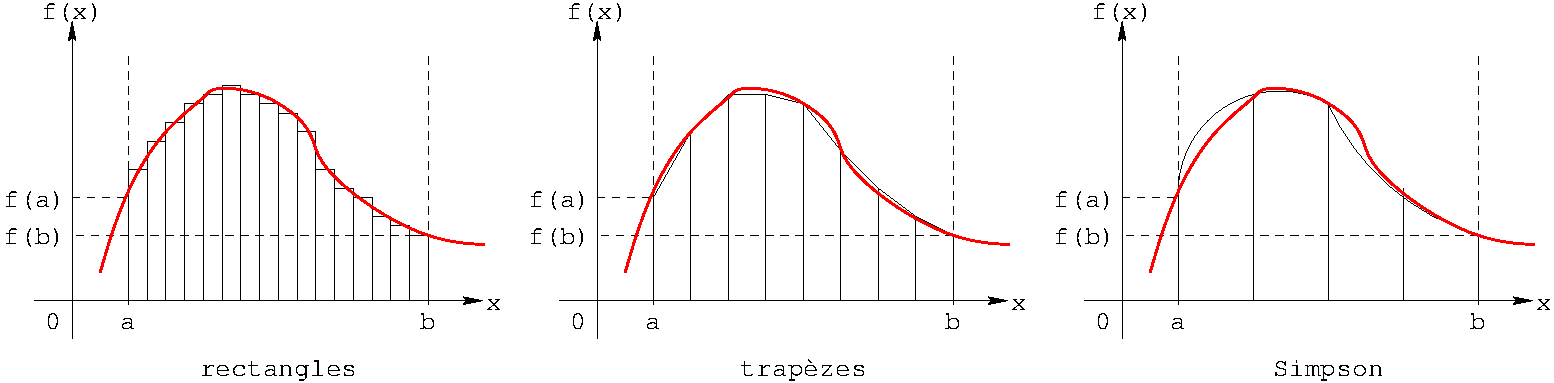
\includegraphics[width=16cm]{integrale.pdf}$$

Dans la méthode des rectangles, on subdivise l'intervalle d'intégration de
	longueur $b-a$ en $n$ parties égales de longueur 
	$\displaystyle\Delta x = \frac{b-a}{n}$. Soient $x_1$, $x_2$, \ldots,
	$x_n$ les points milieux de ces $n$ intervalles. Les $n$ rectangles
	formés avec les ordonnées correspondantes ont pour surface $f(x_1)\Delta
	x$, $f(x_2)\Delta x$, \ldots, $f(x_n)\Delta x$. L'aire sous la courbe 
	est alors assimilée à la somme des aires de ces rectangles, soit 
	$$\displaystyle I = \int_a^b f(x)dx \approx
	\left(f(x_1)+f(x_2)+\cdots+f(x_n)\right)\Delta x = \Delta x \sum_if(x_i)$$ 
	C'est la formule dite
	des rectangles qui repose sur une approximation par une fonction {\em en
	escalier}.
	
	Ecrire un algorithme qui calcule l'intégrale définie $I$ d'une fonction 
	$f$ sur $[a,b]$ à l'ordre $n$ par la méthode des rectangles.

$$\framebox[14.5cm]{$\rule{0cm}{7cm}$}$$
%-----------------------------------------------------------------------------


%-----------------------------------------------------------------------------
\label{fini}
\end{document}
%-----------------------------------------------------------------------------
